\documentclass[russian,utf8,12pt]{eskdtext}
\usepackage[numbertop, numbercenter]{eskdplain}

% - Подключаем шрифты из пакета scalable-cyrfonts-tex
\usepackage{cyrtimes}

% - Отступ красной строки
\setlength{\parindent}{1.25cm}

% - Убирает точку в списке литературы
\makeatletter
\def\@biblabel#1{#1 }

% - Точки для всех пунктов в оглавлении
\renewcommand*{\l@section}{\@dottedtocline{1}{1.5em}{2.3em}}
\renewcommand*{\l@subsection}{\@dottedtocline{1}{1.5em}{2.3em}}
\renewcommand*{\l@subsubsection}{\@dottedtocline{1}{1.5em}{2.3em}}

% - Для переопределения списков
\renewcommand{\theenumi}{\arabic{enumi}}
\renewcommand{\labelenumi}{\theenumi)}
\makeatother

\usepackage{enumitem}
\setlist{nolistsep, itemsep=0.3cm,parsep=0pt}

% - ГОСТ списка литературы
\bibliographystyle{utf8gost705u}

% - Верикальные отступы заголовков 
\ESKDsectSkip{section}{1em}{1em}
\ESKDsectSkip{subsection}{1em}{1em}
\ESKDsectSkip{subsubsection}{1em}{1em}

% - Изменение заголовков
\usepackage{titlesec}
\titleformat{\section}{\centering\normalfont\normalsize}{\thesection}{1.0em}{}
\titleformat{\subsection}{\centering\normalfont\normalsize}{\thesubsection}{1.0em}{}
\titleformat{\subsubsection}{\centering\normalfont\normalsize}{\thesubsubsection}{1.0em}{}
\titleformat{\paragraph}{\centering\normalsize}{\theparagraph}{1.0em}{}

% - Оставим место под ТЗ 
%\setcounter{page}{4}

% - Для больших таблиц
\usepackage{longtable}
\usepackage{tabularx}
\renewcommand{\thetable}{\thesection.\arabic{table}}

% - Используем графику в документе
\usepackage{graphicx}
\graphicspath{{images/}}
\renewcommand{\thefigure}{\thesection.\arabic{figure}}

% - Счётчики
\usepackage{eskdtotal}

% - Выравнивание по ширине
\sloppy

% - Разрешить перенос двух последних букв слова
\righthyphenmin=2

\RequirePackage{enumitem}
\renewcommand{\alph}[1]{\asbuk{#1}}
\setlist{nolistsep}
\setitemize[1]{label=--, fullwidth, itemindent=\parindent, 
  listparindent=\parindent}% для дефисного списка
\setenumerate[1]{label=\arabic*), fullwidth, itemindent=\parindent, 
  listparindent=\parindent}% для нумерованного списка
\setenumerate[2]{label=\alph*), fullwidth, itemindent=\parindent, 
  listparindent=\parindent, leftmargin=\parindent}% для списка 2-ой ступени, который будет нумероваться а), б) и т.д.

\usepackage{listings}  
\lstset{basicstyle=\ttfamily\small}

\begin{document}

\newpage
\ESKDthisStyle{empty}

\begin{center}
 Министерство образования и науки Российской Федерации\\
 Федеральное государственное бюджетное образовательное учреждение высшего профессионального образования\\
 <<ТОМСКИЙ ГОСУДАРСТВЕННЫЙ УНИВЕРСИТЕТ СИСТЕМ УПРАВЛЕНИЯ И РАДИОЭЛЕКТРОНИКИ>> (ТУСУР)\\
 Кафедра комплексной информационной безопасности электронно-вычислительных систем (КИБЭВС)\\
\end{center}

\vfill

\begin{flushright}
\begin{minipage}{0.45\textwidth}
 \begin{flushleft}
  УТВЕРЖДАЮ\\
  заведующий каф. КИБЭВС
  \underline{\hspace{3cm}}А.А. Шелупанов \\
  <<\underline{\hspace{1cm}}>>\underline{\hspace{3cm}}2015г.\\
 \end{flushleft}
\end{minipage}
\end{flushright}

\vfill

\begin{center}
ПРОЕКТИРОВАНИЕ, РАЗРАБОТКА БАЗЫ ДАННЫХ И ПРОГРАММНОГО ОБЕСПЕЧЕНИЯ ДЛЯ ЭЛЕКТРОННОЙ РЕГИСТРАЦИИ НА ПРИЕМ К ВРАЧУ 
(ЭЛЕКТРОННАЯ РЕГИСТРАТУРА)

Курсовая работа по дисциплине <<Безопасность систем баз данных>>

Пояснительная записка к курсовой работе
\end{center}

\vfill
\begin{flushright}
\begin{minipage}{0.45\textwidth}
 \begin{flushleft}
  Выполнила: \\
  студентка гр. 722 \\
  \underline{\hspace{3cm}}М.В. Мейта \\
  <<\underline{\hspace{1cm}}>>\underline{\hspace{3cm}}2015г.\\
 \end{flushleft}
\end{minipage}
\end{flushright}

\vfill

\begin{flushright}
\begin{minipage}{0.45\textwidth}
 \begin{flushleft}
  Научный руководитель: \\
  аспирант каф. КИБЭВС \\
  \underline{\hspace{3cm}}И.В. Горбунов \\
  <<\underline{\hspace{1cm}}>>\underline{\hspace{3cm}}2015г.\\
 \end{flushleft}
\end{minipage}
\end{flushright}

\vfill

\begin{center}
 Томск 2015
\end{center}

\newpage
\ESKDthisStyle{empty}
\paragraph{\hfill РЕФЕРАТ \hfill}
Курсовая работа содержит \ESKDtotal{page} страниц, \ESKDtotal{figure} рисунка, \ESKDtotal{table} таблицы, \ESKDtotal{bibitem} источников, \ESKDtotal{appendix} приложение.

БАЗЫ ДАННЫХ, SQLITE, MONODEVELOP, C#, GTKSharp.

Цель работы --- проектирование, разработка базы данных и клиентской части программного обеспечения для электронной регистрации на прием к врачу (электронная регистратура).

Задачей, поставленной на данный семестр, стало написание программного комплекса, имеющего следующие возможности: 
\begin{enumerate}
\item сбор и анализ событий системных журналов операционной системы;
\item сбор и анализ информации из журналов истории браузеров;
\item сбор и анализ истории переписки мессенджеров;
\item сбор и анализ событий журнальных файлов приложений;
\item поиск файлов по имени.
\end{enumerate}
Результатами работы в данном семестре являются:

\begin{itemize}
\item разработка архитектуры проекта;
\item использование в разработке системы контроля версий GIT;
\item использование Qt --- кроссплатформенной библиотеки С++;
\item изучение вопроса сертификации для возможности внедрения данного комплекса в гос. структуры, занимающиеся информационной безопасностью;
\item использование системы компьютерной вёрстки \TeX для написания документации.
\end{itemize}


Пояснительная записка выполнена при помощи системы компьютерной вёрстки \LaTeX.


\newpage
\ESKDstyle{plain}
\tableofcontents

\newpage
\ESKDstyle{plain}
\section*{Введение}
\addcontentsline{toc}{section}{Введение}
В качестве задания на курсовую работу была поставлена задача разработать базу данных и программу пользователя для осуществления электронной регистрации (записи на прием к врачу) в поликлинике.  


\section{Проектирование инфологической модели данных}
Инфологическая (концептуальная) модель предметной области представляет собой информационную модель наиболее высокого уровня абстракции и в сущности является как образом реальности, так и образом проектируемой базы данных для этой реальности. Она включает в себя описание информационных объектов или понятий предметной области и связей между ними. а также описание ограничений целостности, т.е. требований к допустимым значениям данных и к связям между ними.

Описание бизнесс-процессов в системе электронной регистрации пациентов представлено на диаграммах IDEF0, DFD IDEF3 (рисунки \ref{idef0_1:idef0_1}-\ref{idef3_2:idef3_2}).

\begin{figure}[h!]
\center{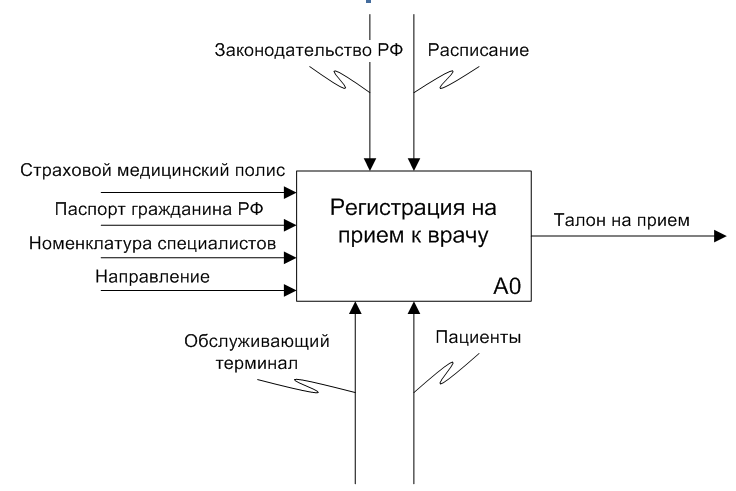
\includegraphics[width=0.5\linewidth]{idef0_1}}
\caption{<<Черный ящик>>}
\label{idef0_1:idef0_1}
\end{figure} 

\begin{figure}[h!]
\center{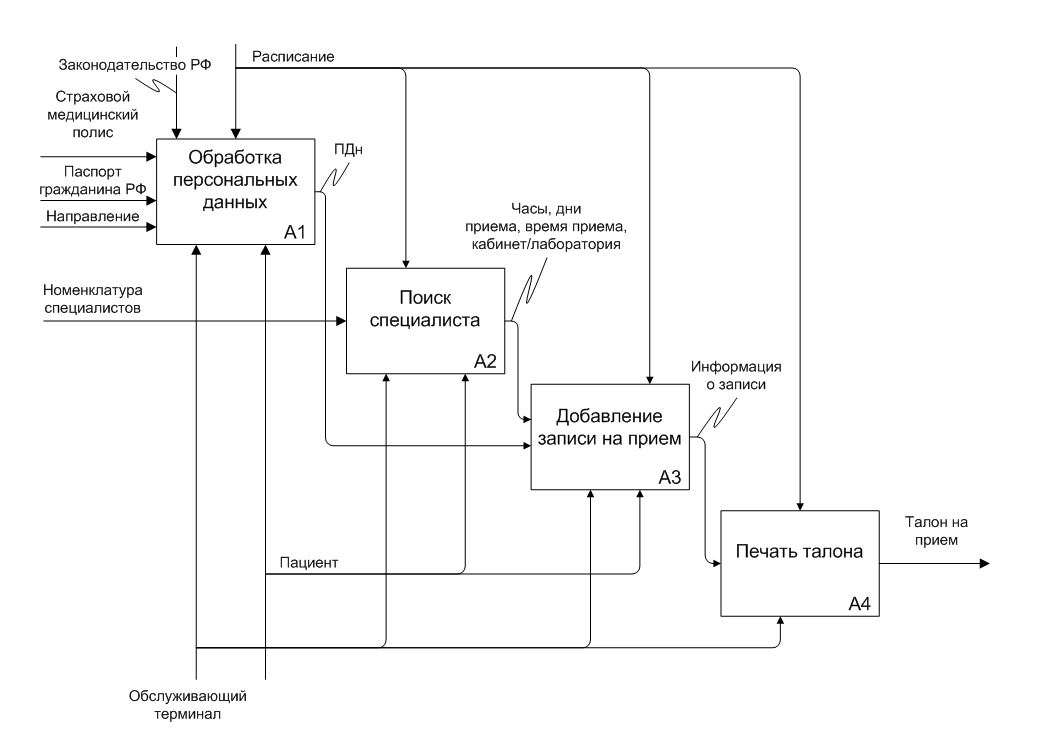
\includegraphics[width=0.9\linewidth]{idef0_2}}
\caption{Диаграмма IDEF0}
\label{idef0_2:idef0_2}
\end{figure} 

\begin{figure}[h!]
\center{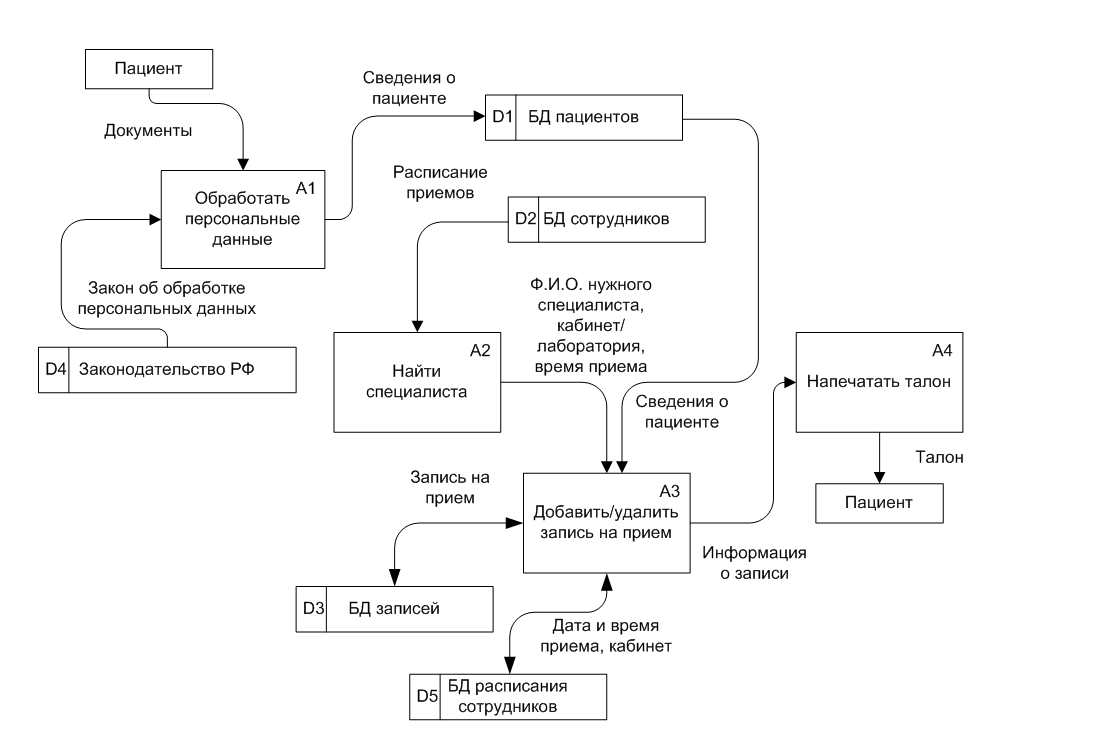
\includegraphics[width=0.9\linewidth]{dfd}}
\caption{DFD-диаграмма бизнес-процессов}
\label{dfd:dfd}
\end{figure} 

\begin{figure}[h!]
\center{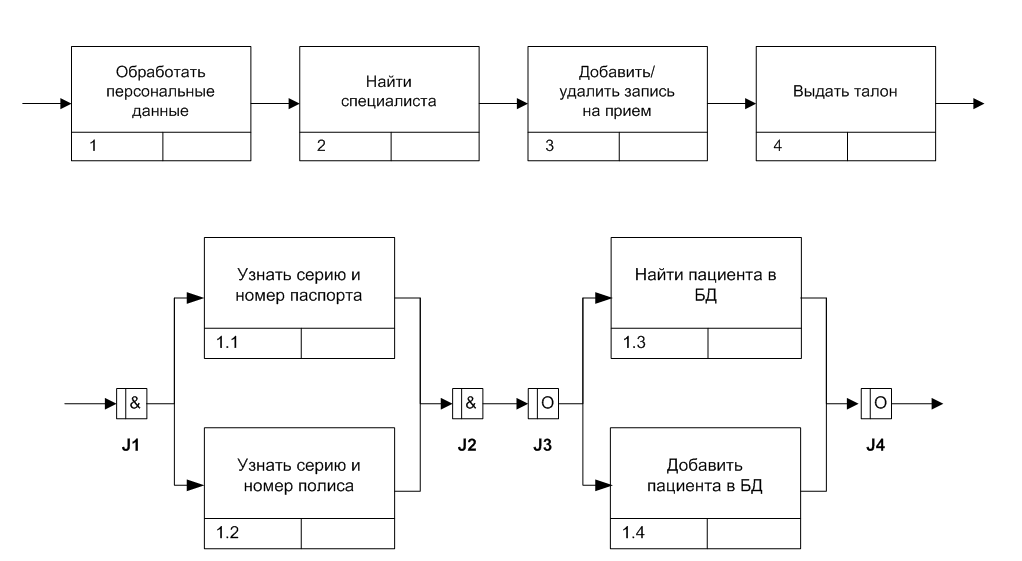
\includegraphics[width=0.9\linewidth]{idef3_1}}
\caption{Диаграмма IDEF3 (часть 1)}
\label{idef3_1:idef3_1}
\end{figure} 

\begin{figure}[h!]
\center{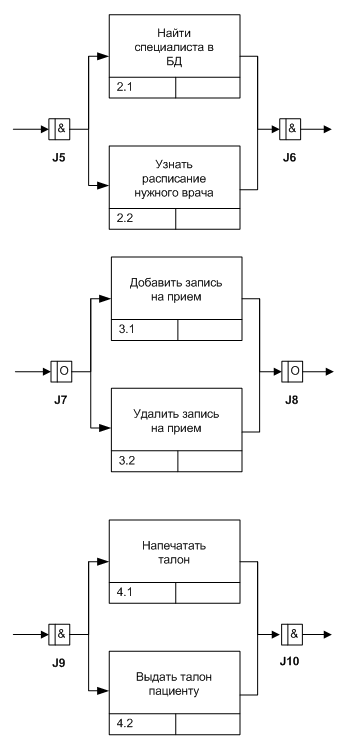
\includegraphics[width=0.4\linewidth]{idef3_2}}
\caption{Диаграмма IDEF3 (часть 2)}
\label{idef3_2:idef3_2}
\end{figure} 

\clearpage






\section{Описание базы данных}
\setcounter{figure}{0}

\subsection{Таблица <<patient>>}
Ограничения на таблицу <<patient>> (пациент):

\begin{itemize}
  \item ID пациента не меньше единицы;
  \item фамилия, имя отчество не должно превосходить 50 символов;
  \item ни один из атрибутов не дожен быть пустым (NULL).
\end{itemize}

\subsection{Таблица <<passport>>}
Ограничения на таблицу <<passport>> (паспорт):

\begin{itemize}
  \item ID пасспорта не меньше единицы;
  \item серия паспорта не должна превосходить 4 символа;
  \item номер паспорта не должен превосходить 6 символов;
  \item адрес места жительства не должен превосходить 100 символов;
  \item атрибут <<пол>> должен состоять из 1 символа (М/Ж);
  \item ни один из атрибутов не дожен быть пустым (NULL).
\end{itemize}

\subsection{Таблица <<policy>>}
Ограничения на таблицу <<policy>> (полис):

\begin{itemize}
  \item ID полиса не меньше единицы;
  \item название страховой медицинской компании не должно превосходить 100 символов;
  \item ни один из атрибутов не дожен быть пустым (NULL).
\end{itemize}

\subsection{Таблица <<talon>>}
Ограничения на таблицу <<talon>> (талон):

\begin{itemize}
  \item ID талона не меньше единицы;
  \item ни один из атрибутов не дожен быть пустым (NULL).
\end{itemize}

\subsection{Таблица <<timetable>>}
Ограничения на таблицу <<timetable>> (расписание):

\begin{itemize}
  \item ID расписания не меньше единицы;
  \item день недели должен состоять из 2-ух символов (<<Пн>>, <<Вт>> и т.д.);
  \item ни один из атрибутов не дожен быть пустым (NULL).
\end{itemize}

\subsection{Таблица <<employee>>}
Ограничения на таблицу <<employee>> (сотрудник):

\begin{itemize}
  \item ID сотрудника не меньше единицы;
  \item специальность сотрудника не должна превосходить 50 символов;
  \item фамилия, имя отчество не должно превосходить 50 символов;
  \item номер рабочего кабинета должен состоять из 3 символов;
  \item ни один из атрибутов не дожен быть пустым (NULL).
\end{itemize}



\section{Описание процесса деятельности} 
\setcounter{figure}{0}

\subsection{Постановка задачи}
\input{problem_form}
\subsection{Описание данных программы}
\input{data_description}
\subsection{Основные технические решения}
\subsubsection{Алгоритм}

Предварительного заполнения базы данных не требуется, однако для возможности добавления записи и регистрации пациента администратору сначала необходимо заполнить базу сотрудников и расписаний.

\begin{center}
  Шаг 1
\end{center}

При авторизации от имени пациента в главном окне программы (MainWindow) появится окно для записи на прием к врачу (EnrollWindow). Необходимо выбрать нужного специалиста, найти его расписание и правильно заполнить предлагаемую форму. Если входные значения были введены неверно, появится сообщение об ошибке. 

\begin{center}
  Шаг 2
\end{center}

Программа проверяет, есть ли уже в БД введенные пользователем серия и номер паспорта. Если данные о пациенте в базе уже есть и форма заполнена верно, появится сообщение об успешной записи, либо сообщение об ошибке записи, если такая запись уже была добавлена в БД.

\begin{center}
  Шаг 3
\end{center}

Если данных о пациенте в базе нет, то появится форма регистрации пациента (PatientRegisterWindow). Если все поля формы заполнены верно, пациент будет добавлен в базу и в окне записи на прием при повторной операции записи появится уведомление об успешном завершении операции, в результате которой будет сгенерирован PDF-файл (талон), готовый к печати.

\begin{center}
  Шаг 4
\end{center}

При авторизации от имени администратора программа сверяет хеш введённого пароля с  хешем, который хранится в БД. Если они совпадают, то открывается окно управления базой данных (AdminWindow), если нет, то появляется уведомление об ошибочной авторизации.

\begin{center}
  Шаг 5
\end{center}

Окно управления базой данных (AdminWindow) позволяет администратору просматривать, удалять и добавлять данные в базу. Для этого необходимо вводить корректные данные, в противном случае операции удаления и добавления выполняться не будут, появится сообщение об ошибке ввода или обращения к базе.

Блок-схема алгоритма работы программы представлена на рисунке~\ref{block:block}.

\begin{figure}[h!]
\center{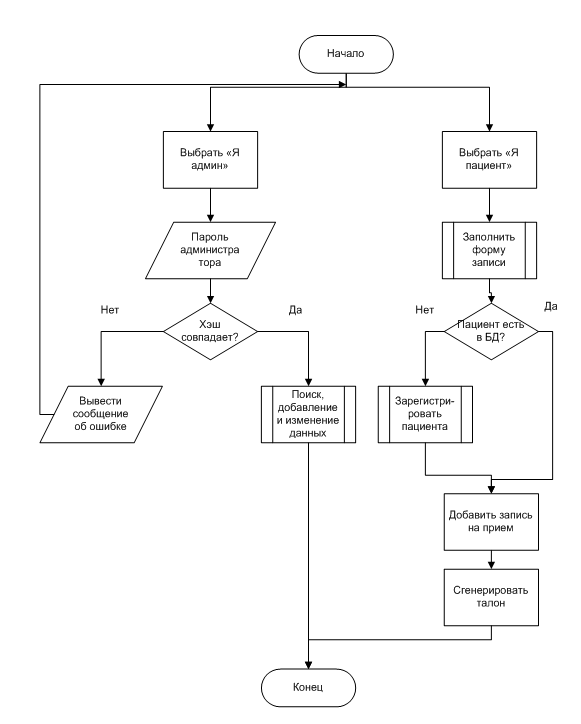
\includegraphics[width=0.8\linewidth]{block}}
\caption{Блок-схема алгоритма работы программы}
\label{block:block}
\end{figure}

\subsubsection{Численность, функции и квалификация персонала}

Для использования системы необходим администратор, который будет добавлять новых сотрудников и менять расписание уже добавленных, следить за целостностью системы, удалять ПДн пациентов по мере необходимости.

\subsubsection{Обеспечение потребительских характеристик системы}

Надежность обеспечивается путем следования стандартам написания кода и использования блоков try-catch для обработки исключительных ситуаций.
Производительность системы обеспечивается путем использования оптимальных алгоритмов.

\subsubsection{Функции, выполняемые системой}

Функциями, выполняемыми программой <<hospital\_register>>, являются регистрация пациентов, добавление записей на прием, печать талонов, управление расписанием и номенклатурой сотрудников (врачей), а также управление записями в БД. 

\subsubsection{Комплекс технических средств}

Для функционирования системы необходимы следующие аппаратные средства:

\begin{itemize}
  \item ОС Linux Ubuntu/Debian;
  \item процессор x86-архитектуры;
  \item объем ОЗУ для выполнения программы: не менее 300 Мб;
  \item объём видеопамяти: не менее 300 Мб;
  \item память на жестком диске: не менее 100 Мб для файлов БД и программы;
  \item монитор с разрешением 800x600 или выше;
  \item мышь, клавиатура;
  \item устройство для чтения CD;
  \item принтер.
\end{itemize}

\subsubsection{Информационное обеспечение системы}

Система поставляется с руководством пользователя и программиста.

\subsubsection{Программное обеспечение системы}

Система разворачивается на компьютере с ОС Linux Ubuntu/Debian.

\section{Мероприятия по подготовке персонала}

Провести ознакомление персонала с руководством пользователя.








\section{Руководство пользователя}
\setcounter{figure}{0}

\section{Перспективы применения программы}
\setcounter{figure}{0}

\section{Заключение}
\setcounter{figure}{0}

% \section{Инструменты}
% \setcounter{figure}{0}
% \subsection{Система контроля версий Git}
% Для разработки программного комплекса для проведения компьютерной экспертизы решено использовать Git.

Git  — распределённая система управления версиями файлов. Проект был создан Линусом Торвальдсом для управления разработкой ядра Linux,  как противоположность  системе управления версиями Subversion (также известная как «SVN») \cite{progit}.

Необходимость использования системы версий, очевидна. Так как в группе несколько программистов и тестер, мы имеем:
\begin{itemize}
\item возможность удаленной работы с исходными кодами;
\item возможность создавать свои ветки, не мешая при этом другим разработчикам;
\item доступ к последним изменениям в коде, т.к. все исходники хранятся на сервере git.keva.su ;
\item исходные коды защищены, доступ к ним можно получить лишь имея RSA-ключ;
\item возможность откатиться к любой стабильной стадии проекта.
\end{itemize}

Основные постулаты работы с кодом в системе Git:

\begin{itemize}
\item каждая задача решается в своей ветке;
\item коммитим сразу, как что-то получили осмысленное;
\item в master мержится не разработчиком, а вторым человеком, который производит вычитку и тестирование изменения;
\item все коммиты должны быть осмысленно подписаны/прокомментированы.
\end{itemize}

Для работы над проектом нами был поднят собственный репозиторий на сервере git.keva.su.
Адреса репозиториев следующие:

Исходные файлы проекта:

git clone git@git.keva.su:gpo.git gpo.git

Репозиторий для тестирования проекта:

git clone git@git.keva.su:gpo-testdata.git gpo-testdata.git

% \subsection{Система компьютерной вёрстки \TeX}
% \TeX\ --- это созданная американским математиком и программистом Дональдом Кнутом система для вёрстки текстов. Сам по себе \TeX\ представляет собой специализированный язык программирования.Каждая издательская система представляет собой пакет макроопределений этого языка.

\LaTeX\ --- это созданная Лэсли Лэмпортом издательская система на базе \TeX'а\cite{lvovskyi}. \LaTeX\ позволяет пользователю сконцентрировать свои услия на содержании и структуре текста, не заботясь о деталях его оформления.

Для подготовки отчётной и иной документации нами был выбран \LaTeX\, так как совместно с системой контроля версий Git он предоставляет возможность совместного создания и редактирования документов. Огромным достоинством системы \LaTeX\ то, что создаваемые с её помощью файлы обладают высокой степенью переносимости \cite{latexrus}.

Совместно с \LaTeX\ часто используется Bib\TeX\ --- программное обеспечение для создания форматированных списков библиографии. Оно входит в состав дистрибутива \LaTeX\ и позволяет создавать удобную, универсальную и долговечную библиографию. Bib\TeX\ стал одной из причин, по которой нами был выбран \LaTeX\ для создания документации.

% \section{Технические характеристики}
% \subsection {Требования к аппаратному обеспечению}

Минимальные системные требования:

\begin{itemize}
\item процессор 1ГГц Pentium 4;
\item оперативная память 512 Мб;
\item место на жёстком диске -- 9 Гб.
\end{itemize}

\subsection {Требования к программному обеспечению}
Для корректной работы разрабатываемого программного комплекса на компьютере должна быть установлена операционная система Debian Squeeze или выше, данная система должна иметь набор библиотек QT.




\newpage
\section*{Заключение}
\addcontentsline{toc}{section}{Заключение}
\textbf{ПРАВИТЬ!!!!!!!!!!!!!!!!!!!!!!!!!!!!!!!!!!!!}

\newpage
\renewcommand{\refname}{Список использованных источников}
\bibliography{lit}

\ESKDappendix{Обязательное}{\normalfont Компакт-диск}
Компакт-диск содержит: 
\begin{itemize}
\item электронную версию пояснительной записки в форматах *.tex и *.pdf;
\item актуальную версию программного комплекса для проведения компьютерной экспертизы;
\item базу данных.
\end{itemize}

\end{document}
